\documentclass[aspectratio=169]{beamer}

\setbeamersize{text margin left=5mm, text margin right=5mm}

\defbeamertemplate{headline}{my header}{%
\vskip1pt%
\makebox[0pt][l]{\,\insertshortauthor}%
\hspace*{\fill}\insertshorttitle/\insertshortsubtitle\hspace*{\fill}%
\llap{\insertpagenumber/\insertpresentationendpage\,}
}
\setbeamertemplate{headline}[my header]

\let\olditem\item
\renewcommand{\item}{\setlength{\itemsep}{\fill}\olditem}

\usepackage{caption}
\usepackage{soul}
\usepackage{tkz-euclide}
\usetikzlibrary{calc}
\usepackage[]{algorithm2e}
\usepackage{changepage}
\usepackage{amssymb}
\usepackage{xcolor}
\usepackage{mathtools}
\usepackage{tcolorbox}
\usepackage{tikz}
\usepackage{tikz-3dplot}
\usetikzlibrary{arrows.meta, decorations.pathreplacing, positioning, shapes.geometric}

%% Fonts
\usefonttheme{professionalfonts}
\usefonttheme{serif}

\DeclareCaptionLabelFormat{blank}{}
\captionsetup[figure]{labelformat=blank}

%% Math definitions
\def\mf{\ensuremath\mathbf}
\def\mb{\ensuremath\mathbb}
\def\mc{\ensuremath\mathcal}
\def\lp{\ensuremath\left(}
\def\rp{\ensuremath\right)}
\def\lv{\ensuremath\left\lvert}
\def\rv{\ensuremath\right\rvert}
\def\lV{\ensuremath\left\lVert}
\def\rV{\ensuremath\right\rVert}
\def\lc{\ensuremath\left\{}
\def\rc{\ensuremath\right\}}
\def\ls{\ensuremath\left[}
\def\rs{\ensuremath\right]}
\def\bmx{\ensuremath\begin{bmatrix*}[r]}
\def\emx{\ensuremath\end{bmatrix*}}
\def\bmxc{\ensuremath\begin{bmatrix*}[c]}
\def\t{\lp t\rp}
\def\k{\ls k\rs}

\newcommand{\demoex}[2]{\onslide<#1->\begin{color}{black!60} #2 \end{color}}
\newcommand{\demoexc}[3]{\onslide<#1->\begin{color}{#2} #3 \end{color}}
\newcommand{\anim}[3]{\onslide<#1->{\begin{color}{#2!60} #3 \end{color}}}
\newcommand{\ct}[1]{\lp #1\rp}
\newcommand{\dt}[1]{\ls #1\rs}
\newcommand{\cols}[2]{\begin{columns}[#1] #2 \end{columns}}
\newcommand{\col}[2]{\begin{column}{#1} #2 \end{column}}

%% Mycolors
\definecolor{myred}{RGB}{192,0,0}
\definecolor{mygray}{RGB}{100,100,100}

%% Custom beamer color
\setbeamercolor{title}{fg=myred}
\setbeamercolor{subtitle}{fg=myred}
\setbeamerfont{title}{series=\bfseries}
% \setbeamercolor{frametitle}{bg=myred, fg=white}
\setbeamercolor{frametitle}{bg=mygray!10!, fg=myred}
\setbeamerfont{frametitle}{series=\bfseries}
\setbeamercolor{item}{fg=mygray}
\setbeamercolor{title in head/foot}{fg=myred}

% Move header to footer
\setbeamertemplate{headline}{}
\setbeamertemplate{footline}{
  \begin{beamercolorbox}[wd=\paperwidth,ht=2.25ex,dp=1ex,center]{footline}
    \inserttitle\hfill\insertauthor\hfill\insertdate\hfill\insertframenumber{}
  \end{beamercolorbox}
}

\title{Applied Linear Algebra in Data Analysis}

% A subtitle is optional and this may be deleted
\subtitle{Concepts in Vector Spaces}

\author{Sivakumar Balasubramanian}
% - Give the names in the same order as the appear in the paper.
% - Use the \inst{?} command only if the authors have different
%   affiliation.

\institute[Christian Medical College] % (optional, but mostly needed)
{
  \inst{}%
  Department of Bioengineering\\
  Christian Medical College, Bagayam\\
  Vellore 632002
}
% - Use the \inst command only if there are several affiliations.
% - Keep it simple, no one is interested in your street address.

\date{}
% - Either use conference name or its abbreviation.
% - Not really informative to the audience, more for people (including
%   yourself) who are reading the slides online

\subject{Lecture notes on ALADA}
% This is only inserted into the PDF information catalog. Can be left
% out. 

% If you have a file called "university-logo-filename.xxx", where xxx
% is a graphic format that can be processed by latex or pdflatex,
% resp., then you can add a logo as follows:

% \pgfdeclareimage[height=0.5cm]{university-logo}{university-logo-filename}
% \logo{\pgfuseimage{university-logo}}

% Delete this, if you do not want the table of contents to pop up at
% the beginning of each subsection:
\AtBeginSubsection[]
{
  \begin{frame}<beamer>{Outline}
    \tableofcontents[currentsection,currentsubsection]
  \end{frame}
}

% Let's get started
\begin{document}

\begin{frame}
  \titlepage
\end{frame}


\begin{frame}[t]{Vectors}
\begin{itemize}
  \item \textbf{Vectors} are ordered list of numbers (scalars). $\mathbf{v} = \begin{bmatrix*}[r] 1.2 \\ -0.1 \\ \vdots \\-1.24 \end{bmatrix*}$.\\
  \textbf{Note:} Small bold letter will represent vectors. e.g. $\mathbf{a}, \mathbf{x}, \ldots $
  
  \item Scalars can be any \textit{field} $\mathbb{R}, \mathbb{C}, \mathbb{Z}, \mathbb{Q}$. Scalars will be represented using lower case normal font, e.g. $x, y, \alpha, \beta, \ldots$
  
  \item Addition/multiplication operations performed on vectors will follow the rules of addition/multiplication of the corresponding scalar fields.
  
  \item We will typically encounter only $\mathbb{R}$ and $\mb{C}$ in this course.
\end{itemize}
\end{frame}


\begin{frame}[t]{Vectors}
\begin{itemize}
  \item Individual elements of a vector $\mathbf{v}$ are indexed. The $i^{th}$ element of $\mathbf{v}$ is referred to as $v_i$.

  \item \textit{Dimension} or \textit{size} of a vector is number of elements in the vector.
  
  \item Set of $n$-real vectors is denoted by $\mathbb{R}^n$ (similarly, $\mathbb{C}^n$)
  
  \item Vectors $\mathbf{a}$ and $\mathbf{b}$ are equal, if
  \begin{itemize}
    \item both have the same size; and
    \item $a_i = b_i, i \in \left\{1, 2, 3, \ldots n\right\}$
  \end{itemize}
  \end{itemize}
\end{frame}


\begin{frame}[t]{Vectors}
\begin{itemize}
\item \textbf{Unit vector} $\mathbf{e}_1 = \begin{bmatrix} 1 \\ 0 \\ 0 \\ \vdots \\ 0 \end{bmatrix}$ \textbf{Zero vector} $\mathbf{0} = \begin{bmatrix} 0 \\ 0 \\ 0 \\ \vdots \\ 0 \end{bmatrix}$ \textbf{One vector} $\mathbf{1} = \begin{bmatrix} 1 \\ 1 \\ 1 \\ \vdots \\ 1 \end{bmatrix}$
\item Geometrically, real $n$-vectors can be thought of as points in $\mathbb{R}^n$ space.\\
\begin{center}
\begin{tikzpicture}
\node (A) at (0,0) {$\mathbf{0}$};
\node (B) at (1,2) {$\mathbf{v}$};
\draw[thick,-latex] (A) -- (B);
\end{tikzpicture}
\end{center}
\end{itemize}
\end{frame}


\begin{frame}[t]{Vectors}
\begin{columns}[T]
\begin{column}{0.5\textwidth}
\begin{itemize}
\item \textbf{Vector scaling}: Multiplication of a scalar and a vector.
\begin{small}
$$ \mathbf{w} = a\mathbf{v} = a\begin{bmatrix} v_1 \\ v_2 \\ v_3 \\ \vdots \\ v_n \end{bmatrix} = \begin{bmatrix} av_1 \\ av_2 \\ av_3 \\ \vdots \\ av_n \end{bmatrix} \,\, a \in \mathbb{R}; \,\, \mathbf{w}, \mathbf{v} \in \mathbb{R}^n$$
\end{small}
\end{itemize}
\begin{center}
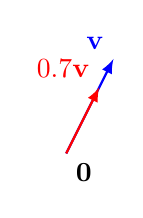
\begin{tikzpicture}[scale=0.6]
\path coordinate (a) at (0,0)
      coordinate (b) at (1.0,2.0)
      coordinate (c) at ($(a)!0.7!(b)$);
\draw[thick,blue,-latex] (a)  -> (b);
\draw[thick,red,-latex] (a)  -> (c);
\node[below right] at (a){$\mathbf{0}$}; 
\node[blue,above left] at (b){$\mathbf{v}$};
\node[red,above left] at (c){$0.7\mathbf{v}$};  
\end{tikzpicture}\hspace{1cm}
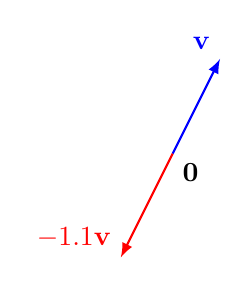
\begin{tikzpicture}[scale=0.6]
\path coordinate (a) at (0,0)
      coordinate (b) at (1.0,2.0)
      coordinate (c) at ($(a)!-1.1!(b)$);
\draw[thick,red,-latex] (a)  -> (c);
\draw[thick,blue,-latex] (a)  -> (b);
\node[below right] at (a){$\mathbf{0}$}; 
\node[blue,above left] at (b){$\mathbf{v}$};
\node[red,above left] at (c){$-1.1\mathbf{v}$};  
\end{tikzpicture}
\end{center}
\end{column}
\begin{column}{0.5\textwidth}
\textbf{Properties}
\begin{itemize}
\item Scalar multiplication is \textit{commutative}.
$$ \alpha \mathbf{v} = \mathbf{v} \alpha $$
\item Scalar multiplication is \textit{associative}.
$$ \left(\alpha \beta\right) \mathbf{v} = \alpha \left(\beta \mathbf{v}\right) $$
\item Scalar multiplication is \textit{distributive}.
$$ \left(\alpha + \beta\right) \mathbf{v} = \alpha \mathbf{v} + \beta \mathbf{v} $$
\end{itemize}
\end{column}
\end{columns}
\end{frame}


\begin{frame}[t]{Vectors}
\begin{columns}[T]
\begin{column}{0.5\textwidth}
\begin{itemize}
\item \textbf{Vector addition}: Adding two vectors of the same dimension, element by element.
\begin{small}
$$ \mathbf{u} + \mathbf{v} = \begin{bmatrix} u_1 \\ u_2 \\ u_3 \\ \vdots \\ u_n \end{bmatrix} + \begin{bmatrix} v_1 \\ v_2 \\ v_3 \\ \vdots \\ v_n \end{bmatrix}= \begin{bmatrix} u_1 + v_1 \\ u_2 + v_2 \\ u_3 + v_3 \\ \vdots \\ u_n + v_n \end{bmatrix} \,\, \mathbf{u}, \mathbf{v} \in \mathbb{R}^n$$
\end{small}
\end{itemize}
\vspace{-0.55cm} 
\begin{center}
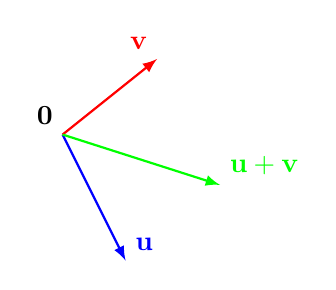
\begin{tikzpicture}[scale=0.8]
\path coordinate (a) at (0,0)
      coordinate (b) at (1.0,-2.0)
      coordinate (c) at (1.5,1.2)
      coordinate (d) at ($(b)!0.5!(c)$)
      coordinate (e) at ($(a)!2.0!(d)$);
\draw[thick,blue,-latex] (a)  -> (b);
\draw[thick,red,-latex] (a)  -> (c);
\draw[thick,green,-latex] (a)  -> (e);
\node[above left] at (a){$\mathbf{0}$}; 
\node[blue,above right] at (b){$\mathbf{u}$};
\node[red,above left] at (c){$\mathbf{v}$};
\node[green,above right] at (e){$\mathbf{u}+\mathbf{v}$};
\end{tikzpicture}
\end{center}
\end{column}
\begin{column}{0.5\textwidth}
\textbf{Properties}
\begin{itemize}
\item Vector addition is \textit{commutative}.
$$ \mathbf{a} + \mathbf{b} = \mathbf{b} + \mathbf{a} $$
\item Vector addition is \textit{associative}.
$$ \left(\mathbf{a} + \mathbf{b}\right) + \mathbf{c} =  \mathbf{a} + \left(\mathbf{b} + \mathbf{c} \right) $$
\item Zero vector has no effect.
$$ \mathbf{a} + \mathbf{0} = \mathbf{a} $$
\item Subtraction of vectors. 
$$ \mathbf{a} + (-1)\mathbf{a} = \mathbf{a} - \mathbf{a} = \mathbf{0} $$
\end{itemize}
\end{column}
\end{columns}
\end{frame}


\begin{frame}[t]{Vector spaces}
\begin{itemize}
\item A set of vectors $V$ that is closed under \textbf{vector addition} and \textbf{vector scaling}.
\[  \forall \mathbf{x}, \mathbf{y} \in V, \,\,\,\, \mathbf{x} + \mathbf{y} \in V \]
\[  \forall \mathbf{x} \in V, \,\,\, \mathrm{and} \,\,\, \alpha \in F, \,\,\,\, \alpha \mathbf{x} \in V \]
\item For a set to be a vector space, it must satisfy the followng properties: $\mathbf{x}, \mathbf{y}, \mathbf{z} \in V$
\begin{itemize}
\item \textit{Commutativity}: $\mathbf{x} + \mathbf{y} = \mathbf{y} + \mathbf{x}$
\item \textit{Associativity of vector addition}: $(\mathbf{x} + \mathbf{y}) + \mathbf{z} = \mathbf{x} + (\mathbf{y} + \mathbf{z})$
\item \textit{Additive identity}: $\mathbf{x} + \mathbf{0} = \mathbf{0} + \mathbf{x} = \mathbf{x}$ $\left(0 \in V\right)$
\item \textit{Additive inverse}: $\exists -\mathbf{x} \in V, \mathbf{x} + (-\mathbf{x}) = \mathbf{0}$
\item \textit{Associativity of scalar multiplication}: $\alpha\left(\beta \mathbf{x}\right) = \left(\alpha\beta \mathbf{x}\right)$
\item \textit{Distributivity of scalar sums}: $\left(\alpha + \beta\right)\mathbf{x} = \alpha \mathbf{x} + \beta \mathbf{x}$
\item \textit{Distributivity of vector sums}: $\alpha\left(\mathbf{x} + \mathbf{y}\right) = \alpha \mathbf{x} + \alpha \mathbf{y}$
\item \textit{Scalar multiplication identity}: $1\mathbf{x} = \mathbf{x}$
\end{itemize}
\item We will mostly deal with $\mathbb{R}^n$ and $\mb{C}^n$ vectors spaces in this course.
\end{itemize}
\end{frame}

\begin{frame}[t]{Subspaces}
\begin{itemize}
    \item A \textbf{subspace} $S$ of a vector space $V$ is a subset of $V$ and is itself a vector space.
    \[ S \subset V, \,\,\,\, \forall \mathbf{x}, \mathbf{y} \in S, \alpha \mathbf{x} + \beta \mathbf{y} \in S, \,\,\, \alpha, \beta \in F \]
    \item The zero vector is called the \textbf{trivial subspace} of a vector space $V$.
    \item For example, in $\mathbb{R}^3$ all planes and lines passing through the origin are subspaces of $\mathbb{R}^3$. 
\end{itemize}
\begin{center}
\tdplotsetmaincoords{70}{110}
\begin{tikzpicture}[scale=2,tdplot_main_coords]
    \def\x{.75}
    \filldraw[draw=white, fill=blue!20] (\x, 0, \x)-- (\x, 0, {-1*\x})-- ({-1*\x}, 0, {-1*\x})-- ({-1*\x}, 0, \x)-- cycle;
    \draw[thick,-latex] (0,0,0) -- (1.5,0,0) node[anchor=north east]{$x$};
    \draw[thick,-latex] (0,0,0) -- (0,1,0) node[anchor=north west]{$y$};
    \draw[thick,-latex] (0,0,0) -- (0,0,1) node[anchor=south]{$z$};
    \draw[thin,dashed] (0,0,0) -- (-0.75,0,0);
    \draw[thin,dashed] (0,0,0) -- (0,-0.5,0);
    \draw[thin,dashed] (0,0,0) -- (0,0,-0.5);

    \draw[thick, red, -] (-1,-1,0) -- (1,1,0);
\end{tikzpicture}
\end{center}
\end{frame}


\begin{frame}[t]{Linear independence}
\begin{itemize}
  \item A collection of vectors $\left\{\mathbf{x}_1, \mathbf{x}_2, \mathbf{x}_3, \ldots \mathbf{x}_n\right\}, \,\,\, \mathbf{x}_i \in \mathbb{R}^m \,\,\, i \in\left\{1, 2, 3, \ldots n\right\}$ is called \textit{linearly dependent} if,
  $$ \sum_{i=1}^n\alpha_i\mathbf{x}_i = 0, \text{ hold for some } \alpha_1, \alpha_2, \ldots \alpha_n \in \mathbb{R}, \text{ such that } \exists \alpha_i \neq 0 $$
  
  \item Another way to state this: A collection of vectors is \textit{linearly dependent} if at least one of the vectors in the collection can be expressed as a linear combination of the other vectors in the collection, i.e.
  $$\mathbf{x}_i = -\sum_{j=1, j\neq i}^{n}\left(\frac{\alpha_j}{\alpha_i}\right)\mathbf{x}_j$$
\end{itemize}
\end{frame}


\begin{frame}[t]{Linear independence}
\begin{itemize}  
  \item A collection of vectors is \textit{linearly independent} if it is \textbf{not} \textit{linearly dependent}.
  $$ \sum_{i=1}^n\alpha_i\mathbf{x}_i = 0 \implies \alpha_1=\alpha_2=\alpha_3\ldots=\alpha_n = 0$$
\end{itemize}
\end{frame}


\begin{frame}[t]{Span of a set of vectors}
\begin{itemize}
    \item Consider a set of vectors $S = \left\{\mathbf{v}_1, \mathbf{v}_2, \mathbf{v}_3 \ldots \mathbf{v}_r\right\}$ where $\mathbf{v}_i \in \mathbb{R}^n, 1 \leq i \leq r$.
    \item The \textbf{span} of the set $S$ is defined as the set of all linear combinations of the vectors $\mathbf{v}_i$,
    \[ span\left(S\right) = \left\{\alpha_1\mathbf{v}_1 + \alpha_2\mathbf{v}_2 + \ldots + \alpha_r\mathbf{v}_r\right\}, \,\, \alpha_i \in \mathbb{R} \]
    \item Is $span\left(S\right)$ a subspace of $\mathbb{R}^n$?
\end{itemize}
\end{frame}


\begin{frame}[t]{Span of a set of vectors}
\begin{itemize}
    \item We say that the subspace $span\left(S\right)$ is spanned by the \textit{spanning set} $S$. $\longrightarrow$ $S$ \textit{spans} $span\left(S\right)$.
    \item \textbf{Sum of subspaces} $X, Y$ is defined as the sum of all possible vectors from $X$ and $Y$.
    \[ X + Y = \left\{\mathbf{x} + \mathbf{y} \left|\right. \mathbf{x} \in X, \mathbf{y} \in Y\right\} \]
    \item Sum of two subspace is also a subspace.
\end{itemize}
\end{frame}


\begin{frame}[t]{Inner Product}
\begin{itemize}
    \item \textbf{Standard inner product} is defined as the following,
    $$\mathbf{x}^\top\mathbf{y} = \sum_{i=1}^{n}x_iy_i, \,\,\, \mathbf{x}, \mathbf{y} \in \mathbb{R}^n$$\\
    For complex vectors:  $\mathbf{x}^{*}\mathbf{y} = \sum_{i=1}^{n}\overline{x}_iy_i, \,\,\, \mathbf{x}, \mathbf{y} \in \mathbb{C}^n$
    \item \textbf{Properties}
    \begin{itemize}
        \item $\mathbf{x}^\top\mathbf{x} > 0, \,\,\, \forall \mathbf{x} \neq 0$ and $\mathbf{x}^\top\mathbf{x} = 0 \Leftrightarrow \mathbf{x} = 0$
        \item \textit{Commutative}: $\mathbf{x}^\top\mathbf{y} = \mathbf{y}^\top\mathbf{x}$
        \item \textit{Associativity with scalar multiplication}: $\left(\alpha \mathbf{x}\right)^\top\mathbf{y} = \alpha \left(\mathbf{x}^\top\mathbf{y}\right)$
        \item \textit{Distributivity with vector addition}: $\left(\mathbf{x} + \mathbf{y}\right)^\top\mathbf{z} = \mathbf{x}^\top\mathbf{z} + \mathbf{y}^\top\mathbf{z}$
    \end{itemize}
\end{itemize}
\end{frame}


\begin{frame}[t]{Norm}
\begin{columns}[T]
\begin{column}{0.65\textwidth}
\vspace{-0.5cm}
\begin{small}
\begin{itemize}
  \item Norm is a measure of the size of a vector.
  \item \textit{Euclidean norm} of a $n$-vector $\mathbf{x} \in \mathbb{R}^n$ is defined as, $\left\Vert \mathbf{x}\right\Vert_2 = \sqrt{\mathbf{x}^\top\mathbf{x}} = \sqrt{\sum_{i=1}^{n}x_i^2}$.
  \item $\left\Vert \mathbf{x} \right\Vert_2$ is a measure of the length of the vector $\mathbf{x}$.
  \item Any function of the form $\left\Vert\bullet\right\Vert: \mathbb{R}^n \longrightarrow \mathbb{R}_{\geq 0}$ is a valid norm, provided it satisfies the following properties.
\end{itemize}
\end{small}
\end{column}
\begin{column}{0.35\textwidth}
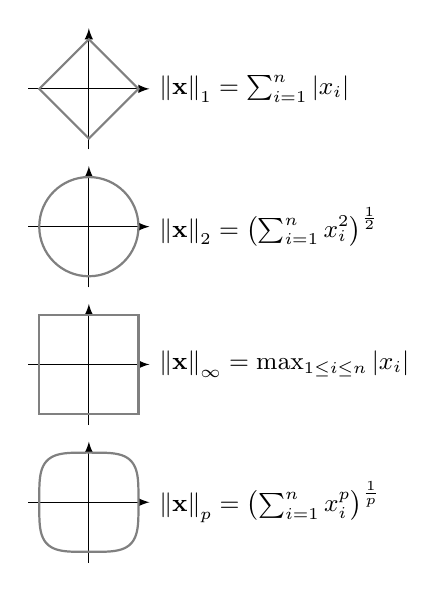
\begin{tikzpicture}[scale=0.7]
  \def \r{0.9}
  \def \ya{0}
  \def \yb{-2.5}
  \def \yc{-5}
  \def \yd{-7.5}
  
  \draw[-latex] (3.9,\ya) -- (6.1,\ya) node[black,right,xshift=0.cm, yshift=0.cm] {\small{$\left\Vert \mathbf{x} \right\Vert_1 = \sum_{i=1}^{n}\left|x_i\right|$}};
  \draw[-latex] (5,\ya-1.1) -- (5,\ya+1.1);
  \draw[thick, gray] (5-\r,0)--(5,\r)--(5+\r,0)--(5,-\r)--cycle;
  
  \draw[-latex] (3.9,\yb) -- (6.1,\yb) node[black,right,xshift=0.cm, yshift=0.cm] {\small{$\left\Vert \mathbf{x} \right\Vert_2 = \left(\sum_{i=1}^{n}x_i^2\right)^{\frac{1}{2}}$}};
  \draw[-latex] (5,\yb-1.1) -- (5,\yb+1.1);
  \draw [thick, gray](5,-2.5) circle (\r);
  
  \draw[-latex] (3.9,\yc) -- (6.1,\yc) node[black,right,xshift=0.cm, yshift=0.cm] {\small{$\left\Vert \mathbf{x} \right\Vert_\infty = \max_{1\leq i\leq n}\left|x_i\right|$}};
  \draw[-latex] (5,\yc-1.1) -- (5,\yc+1.1);
  \draw[thick, gray] (5-\r,-5-\r)--(5-\r,-5+\r)--(5+\r,-5+\r)--(5+\r,-5-\r)--cycle;

  \draw[-latex] (3.9,\yd) -- (6.1,\yd) node[black,right,xshift=0.cm, yshift=0.cm] {\small{$\left\Vert \mathbf{x} \right\Vert_p = \left(\sum_{i=1}^{n}x_i^p\right)^{\frac{1}{p}}$}};
  \draw[-latex] (5,\yd-1.1) -- (5,\yd+1.1);
  \draw[thick, gray,scale=1,domain=0:90,samples=100,smooth,variable=\t]
  plot({-\r*sqrt(cos(\t))+5},{\r*sqrt(sin(\t))-7.5});
  \draw[thick, gray,scale=1,domain=0:90,samples=100,smooth,variable=\t]
  plot({-\r*sqrt(cos(\t))+5},{-\r*sqrt(sin(\t))-7.5});
  \draw[thick, gray,scale=1,domain=0:90,samples=100,smooth,variable=\t]
  plot({\r*sqrt(cos(\t))+5},{-\r*sqrt(sin(\t))-7.5});
  \draw[thick, gray,scale=1,domain=0:90,samples=100,smooth,variable=\t]
  plot({\r*sqrt(cos(\t))+5},{\r*sqrt(sin(\t))-7.5});                 
\end{tikzpicture}
\end{column}
\end{columns}
\end{frame}


\begin{frame}[t]{Norm}
\begin{columns}[T]
\begin{column}{0.65\textwidth}
\vspace{-0.5cm}
\begin{small}
\begin{itemize}
  \item \textbf{Properties}
  \begin{itemize}
  \item \textit{Definiteness}. $\left\Vert \mathbf{x}\right\Vert = 0 \iff x = 0$
  \item \textit{Non-negativity}. $\left\Vert \mathbf{x} \right\Vert \geq 0$
  \item \textit{Non-negative homogeneity}. $\left\Vert \beta \mathbf{x} \right\Vert = \left|\beta\right|\left\Vert \mathbf{x} \right\Vert, \, \beta \in \mathbb{R}$
  \item \textit{Triangle inequality}. $\left\Vert \mathbf{x} + \mathbf{y}\right\Vert \leq \left\Vert \mathbf{x}\right\Vert + \left\Vert \mathbf{y}\right\Vert$
  \end{itemize}
  \item $p$-norm: $\left\Vert \mathbf{x} \right\Vert_p = \left(\sum_{i=1}^{n}\left|x_i\right|^p\right)^{\frac{1}{p}}$
  \item Norm of difference between two vectors is a measure of the distance between the vectors. $d = \left\Vert \mathbf{x} - \mathbf{y} \right\Vert_2$.
\end{itemize}
\end{small}
\end{column}
\begin{column}{0.35\textwidth}
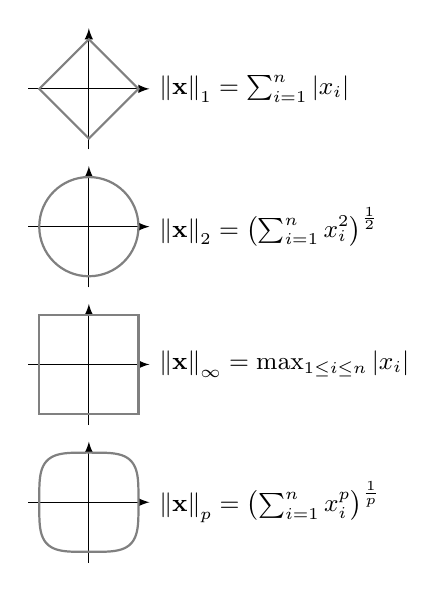
\begin{tikzpicture}[scale=0.7]
  \def \r{0.9}
  \def \ya{0}
  \def \yb{-2.5}
  \def \yc{-5}
  \def \yd{-7.5}
  
  \draw[-latex] (3.9,\ya) -- (6.1,\ya) node[black,right,xshift=0.cm, yshift=0.cm] {\small{$\left\Vert \mathbf{x} \right\Vert_1 = \sum_{i=1}^{n}\left|x_i\right|$}};
  \draw[-latex] (5,\ya-1.1) -- (5,\ya+1.1);
  \draw[thick, gray] (5-\r,0)--(5,\r)--(5+\r,0)--(5,-\r)--cycle;
  
  \draw[-latex] (3.9,\yb) -- (6.1,\yb) node[black,right,xshift=0.cm, yshift=0.cm] {\small{$\left\Vert \mathbf{x} \right\Vert_2 = \left(\sum_{i=1}^{n}x_i^2\right)^{\frac{1}{2}}$}};
  \draw[-latex] (5,\yb-1.1) -- (5,\yb+1.1);
  \draw [thick, gray](5,-2.5) circle (\r);
  
  \draw[-latex] (3.9,\yc) -- (6.1,\yc) node[black,right,xshift=0.cm, yshift=0.cm] {\small{$\left\Vert \mathbf{x} \right\Vert_\infty = \max_{1\leq i\leq n}\left|x_i\right|$}};
  \draw[-latex] (5,\yc-1.1) -- (5,\yc+1.1);
  \draw[thick, gray] (5-\r,-5-\r)--(5-\r,-5+\r)--(5+\r,-5+\r)--(5+\r,-5-\r)--cycle;

  \draw[-latex] (3.9,\yd) -- (6.1,\yd) node[black,right,xshift=0.cm, yshift=0.cm] {\small{$\left\Vert \mathbf{x} \right\Vert_p = \left(\sum_{i=1}^{n}x_i^p\right)^{\frac{1}{p}}$}};
  \draw[-latex] (5,\yd-1.1) -- (5,\yd+1.1);
  \draw[thick, gray,scale=1,domain=0:90,samples=100,smooth,variable=\t]
  plot({-\r*sqrt(cos(\t))+5},{\r*sqrt(sin(\t))-7.5});
  \draw[thick, gray,scale=1,domain=0:90,samples=100,smooth,variable=\t]
  plot({-\r*sqrt(cos(\t))+5},{-\r*sqrt(sin(\t))-7.5});
  \draw[thick, gray,scale=1,domain=0:90,samples=100,smooth,variable=\t]
  plot({\r*sqrt(cos(\t))+5},{-\r*sqrt(sin(\t))-7.5});
  \draw[thick, gray,scale=1,domain=0:90,samples=100,smooth,variable=\t]
  plot({\r*sqrt(cos(\t))+5},{\r*sqrt(sin(\t))-7.5});                 
\end{tikzpicture}
\end{column}
\end{columns}
\end{frame}


\begin{frame}[t]{Orthogonality}
\begin{itemize}
\item Orthogonality is the idea of two vectors being perpendicular, $\mathbf{x} \perp \mathbf{y}$.
\begin{center}
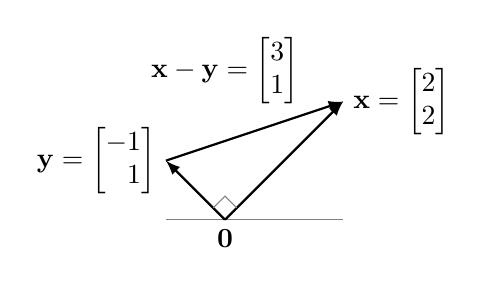
\begin{tikzpicture}[scale=0.75]
  \node[black, below] at (0, 0) {$\mathbf{0}$};
  \draw[gray,thin,-] (-1, 0) -- (2, 0) ;
  \draw[black,thick,-latex] (0, 0) -- (2, 2) node[black, above, right]{$\mathbf{x}=\begin{bmatrix*}[r]2\\2\end{bmatrix*}$};
  \draw[black,thick,-latex] (0, 0) -- (-1, 1) node[black, above, left]{$\mathbf{y}=\begin{bmatrix*}[r]-1\\1\end{bmatrix*}$};
  \draw[black,thick,-latex] (-1, 1) -- (2, 2) node[black, yshift=0.40cm, xshift=-1.5cm]{$\mathbf{x}-\mathbf{y}=\begin{bmatrix*}[r]3\\1\end{bmatrix*}$};
  \draw [gray,thin](0.2,0.2) -- (0, 0.4) -- (-0.2, 0.2);
\end{tikzpicture}
\end{center}

Using the Pythagonean theorem,  $\left\lVert \mathbf{x} - \mathbf{y}\right\rVert^2 = \left\lVert \mathbf{x}\right\rVert^2 + \left\lVert \mathbf{y}\right\rVert^2$
\[ \left\lVert \mathbf{x}\right\rVert^2 + \left\lVert \mathbf{y}\right\rVert^2 - 2 \mathbf{x}^\top\mathbf{y} = \left\lVert \mathbf{x}\right\rVert^2 + \left\lVert \mathbf{y}\right\rVert^2 \implies \mathbf{x}^\top\mathbf{y} = 0 \]

\item We extend this to the $n$-dimensional case and define two vectors $\mathbf{x}, \mathbf{y} \in \mathbb{R}^n$ being orthogonal, if
\[ \mathbf{x}^\top\mathbf{y} = \sum_{i=1}^{n}x_iy_i = 0\]
\end{itemize}
\end{frame}


\begin{frame}[t]{Angle between vectors}
\vspace{-0.5cm}
\begin{center}
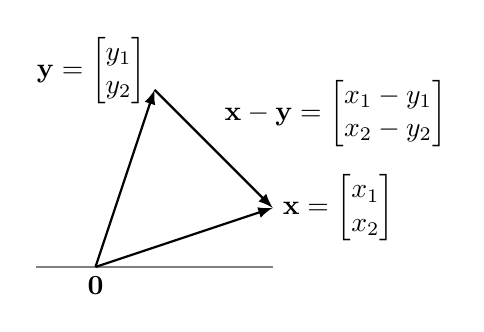
\begin{tikzpicture}[scale=0.75]
  \node[black, below] at (0, 0) {$\mathbf{0}$};
  \draw[gray,thin,-] (-1, 0) -- (3, 0) ;
  \draw[black,thick,-latex] (0, 0) -- (3, 1) node[black, above, right]{$\mathbf{x} = \begin{bmatrix*}x_1\\x_2\end{bmatrix*}$};
  \draw[black,thick,-latex] (0, 0) -- (1, 3) node[black, yshift=0.25cm, xshift=-0.8cm]{$\mathbf{y} = \begin{bmatrix*}y_1\\y_2\end{bmatrix*}$};
  \draw[black,thick,-latex] (1, 3) -- (3, 1) node[black, xshift=0.8cm, yshift=1.2cm]{$\mathbf{x} - \mathbf{y} = \begin{bmatrix*}x_1-y_1\\x_2-y_2\end{bmatrix*}$};
  % \draw[gray,domain=20:70] plot({0.75 * cos(\x)}, {0.75 * sin(\x)});
  % \node[gray, below] at (0.75, 1.0) {{\footnotesize $\theta$}};
  % \draw[blue,domain=0:19] plot({1.0 * cos(\x)}, {1.0 * sin(\x)});
  % \node[blue, yshift=0.15cm] at (1.3, 0.0) {{\footnotesize $\beta$}};
  % \draw[red,domain=0:70] plot({0.5 * cos(\x)}, {0.5 * sin(\x)});
  % \node[red, yshift=0.18cm] at (0.23, 0.0) {{\footnotesize $\alpha$}};
  % \node[right] at (7,3.5) {$\cos \alpha = \frac{y_1}{\left\lVert \mathbf{y}\right\rVert}, \,\,\, \cos \beta = \frac{x_1}{\left\lVert \mathbf{x}\right\rVert}$};
  % \node[right] at (7,2.5) {$\sin \alpha = \frac{y_2}{\left\lVert \mathbf{y}\right\rVert}, \,\,\, \sin \beta = \frac{x_2}{\left\lVert \mathbf{x}\right\rVert}$};
  % \node[right] at (7,1.5) {$\cos \left(\alpha - \beta\right) = \cos \alpha \cos \beta + \sin \alpha \cos \beta$};
  % \node[right] at (7,0.5) {$\cos \left(\theta\right) = \frac{x_1y_1 + x_2y_2}{\left\lVert \mathbf{x}\right\rVert \left\lVert \mathbf{y}\right\rVert} = \frac{\mathbf{x}^\top\mathbf{y}}{\left\lVert \mathbf{x}\right\rVert \left\lVert \mathbf{y}\right\rVert}$};
  % \node[right] at (7,-0.5) {$\mathbf{x}^\top\mathbf{y} = \left\lVert \mathbf{x}\right\rVert \left\lVert \mathbf{y}\right\rVert \cos \left(\theta\right)$};
\end{tikzpicture}
\end{center}

\vspace{-0.5cm}
\begin{itemize}
    \item Inner products are used for projecting a vector onto another vector or a subspace.
    \item It is also a measure of similarity between two vectors, $\cos \left(\theta\right) = \frac{\mathbf{x}^\top\mathbf{y}}{\left\lVert \mathbf{x}\right\rVert \left\lVert \mathbf{y}\right\rVert}$
    \item \textbf{Cauchy-Bunyakovski-Schwartz Inequality}:
    \[ \left\lvert \mathbf{x}^\top\mathbf{y} \right\rvert \leq \left\lVert \mathbf{x} \right\rVert \left\lVert \mathbf{y} \right\rVert, \,\,\, \mathbf{x}, \mathbf{y} \in \mathbb{R}^n \]
\end{itemize}
\end{frame}


\begin{frame}[t]{Basis}
  \begin{small}
  \noindent Consider a vector $\mathbf{y} = \sum_{i=1}^n\alpha_i\mathbf{x}_i$. What can we say about the coefficients $\alpha_i$s when the collection $\left\{\mathbf{x}_i\right\}_{i=1}^n$ is,
  \begin{itemize}
  \item linearly independent $\implies \alpha_i$s are \textit{unique}.
  \item linearly dependent $\implies \alpha_i$s are not \textit{unique}.
  \end{itemize}
  
  Consider $\mathbb{R}^2$ vector space. $\mathbf{x}_1=\begin{bmatrix}1\\0\end{bmatrix}, \,\, \mathbf{x}_2=\begin{bmatrix}1\\1\end{bmatrix} \,\, \mathbf{x}_3 = \begin{bmatrix}-1\\1\end{bmatrix}$.
  \begin{center}
  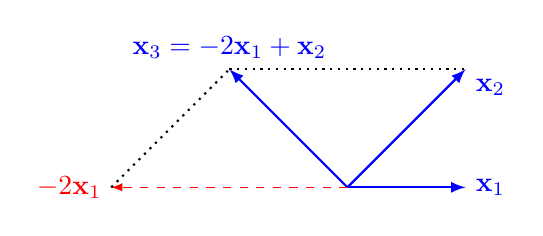
\begin{tikzpicture}[scale=1.5]
    \draw[thick, blue, -latex] (0,0) -- (1, 0) node[right]{$\mathbf{x}_1$};
    \draw[thick, blue, -latex] (0,0) -- (1, 1) node[below right]{$\mathbf{x}_2$};
    \draw[thick, blue, -latex] (0,0) -- (-1, 1) node[above]{$\mathbf{x}_3 = -2\mathbf{x}_1 + \mathbf{x}_2$};
    \draw[dashed, red, -latex] (0,0) -- (-2, 0) node[left]{$-2\mathbf{x}_1$};
    \draw[dotted, thick, black] (-2,0) -- (-1, 1);
    \draw[dotted, thick, black] (-1,1) -- (1, 1);
  \end{tikzpicture}
  \end{center}
  \noindent \textbf{Independence-Dimension inequality}: What is the maximum possible size of a linearly independent collection?
  \begin{center}\textit{A linearly independent collection of n-vectors can at most have n vectors.}\end{center}
  \end{small}
  \end{frame}
  
  
\begin{frame}[t]{Basis}
How many vectors can we choose from the following vectors before the set becomes linearly dependent?
  
  \begin{center}
  \begin{center}
  \tdplotsetmaincoords{70}{110}
  \begin{tikzpicture}[scale=3,tdplot_main_coords]
      \def\x{.75}
      \filldraw[draw=white, fill=blue!20] (\x, 0, \x)-- (\x, 0, {-1*\x})-- ({-1*\x}, 0, {-1*\x})-- ({-1*\x}, 0, \x)-- cycle;
      \draw[thick,-latex] (0,0,0) -- (1.5,0,0) node[anchor=north east]{$x$};
      \draw[thick,-latex] (0,0,0) -- (0,1,0) node[anchor=north west]{$y$};
      \draw[thick,-latex] (0,0,0) -- (0,0,1) node[anchor=south]{$z$};
      \draw[thin,dashed] (0,0,0) -- (-0.75,0,0);
      \draw[thin,dashed] (0,0,0) -- (0,-0.5,0);
      \draw[thin,dashed] (0,0,0) -- (0,0,-0.5);
      \draw[thick, red, -] (-1,-1,0) -- (1,1,0);
  \end{tikzpicture}
  \end{center}
  \end{center}
\end{frame}
  
  
\begin{frame}[t]{Basis}
  \begin{itemize}
    \item A linearly independent set of $n$-vectors from $\mathbb{R}^n$, of size $n$, is called a \textit{basis} for $\mathbb{R}^n$.
  
    \item Any $n$-vector from $\mathbb{R}^n$ can be represented as a \textit{unique} linear combination of the elements of the basis.
    
    \item Consider the basis $\left\{\mathbf{x}_i\right\}_{i=1}^{n}$, $\mathbf{x}_i \in \mathbb{R}^n$. Any vector $\mathbf{y} \in \mathbb{R}^n$ can be represented as a linear combination of $\mathbf{x}_i$s, $\mathbf{y} = \sum_{i=1}^n \alpha_i\mathbf{x}_i$. This is called the \textit{expansion of} $\mathbf{y}$ in the $\left\{\mathbf{x}_i\right\}_{i=1}^n$ basis.
  \end{itemize}
\end{frame}
  
  
  \begin{frame}[t]{Basis}
  \begin{itemize}
    \item The numbers $\alpha_i$ are called the \textit{coefficients} of the expansion of $\mathbf{y}$ in the $\left\{\mathbf{x}_i\right\}_{i=1}^n$ basis.
    
    \item \textbf{Orthogonal vectors}: A set of vectors $\left\{\mathbf{x}_i\right\}_{i=1}^n$ is \textit{(mutually) orthogonal} if $\mathbf{x}_i \perp \mathbf{x}_j$ for all $i, j \in \left\{1, 2, 3, \ldots n\right\}$ and $i \neq j$.
    
    \item This set is called \textbf{orthonormal} if its elements are all of unit length $\left\Vert \mathbf{x}_i \right\Vert_2 = 1$ for all $i \in \left\{1, 2, 3, \ldots n\right\}$.
  \end{itemize}
  \[ \mathbf{x}_i^\top\mathbf{x}_j = \begin{cases} 
        0 & i \neq j \\
        1 & i = j 
     \end{cases}
  \]
  \end{frame}
  
  
  \begin{frame}[t]{Representing a Vector in an Orthonormal Basis}
  \begin{itemize}
  \item An orthonormal collection of vectors is linearly independent.
  \item Consider an orthonormal basis $\left\{\mathbf{x}_i\right\}_{i=1}^{n}$. The expansion of a vector $\mathbf{y}$ is given by,
  \[ \mathbf{y} = \alpha_1\mathbf{x}_1 + \alpha_2\mathbf{x}_2 + \alpha_3\mathbf{x}_3 + \ldots + \alpha_n\mathbf{x}_n \]
  \[ \mathbf{x}_i^\top\mathbf{y} = \alpha_1\mathbf{x}_i^\top\mathbf{x}_1 + \alpha_2\mathbf{x}_i^\top\mathbf{x}_2 + \alpha_3\mathbf{x}_i^\top\mathbf{x}_3 + \ldots + \alpha_n\mathbf{x}_i^\top\mathbf{x}_n = \alpha_i\]
  \end{itemize}
  \end{frame}
  
  \begin{frame}[t]{Representing a Vector in an Orthonormal Basis}
  \begin{itemize}
  \item Thus, we can rewrite this as,
  \[ \mathbf{y} = \left(\mathbf{y}^\top\mathbf{x}_1\right)\mathbf{x}_1 + \left(\mathbf{y}^\top\mathbf{x}_2\right)\mathbf{x}_2 + \left(\mathbf{y}^\top\mathbf{x}_3\right)\mathbf{x}_3 + \ldots + \left(\mathbf{y}^\top\mathbf{x}_n\right)\mathbf{x}_n \]
  \end{itemize}
  \begin{center}
  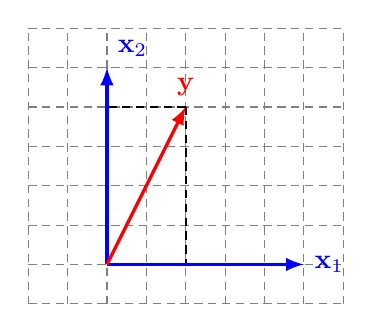
\begin{tikzpicture}[scale=2.5]
    \foreach \x in {-0.4, -0.2, 0, 0.2, 0.4, 0.6, 0.8, 1.0, 1.2}
      \draw[gray, thin, densely dashed] (\x,-0.2)--(\x,1.2);
    \foreach \x in {-0.2, 0, 0.2, 0.4, 0.6, 0.8, 1.0, 1.2}
      \draw[gray, thin, densely dashed] (-0.4,\x)--(1.2,\x);
    \draw[thick, densely dashed, black] (0.4,0.8) -- (0.4,0);
    \draw[thick, densely dashed, black] (0.4,0.8) -- (0.,0.8);
    \draw[very thick, blue, -latex] (0,0) -- (1,0) node[right]{$\mathbf{x}_1$};
    \draw[very thick, blue, -latex] (0,0) -- (0,1) node[above right]{$\mathbf{x}_2$};
    \draw[very thick, red, -latex] (0,0) -- (0.4,0.8) node[above]{$\mathbf{y}$};
  \end{tikzpicture}
  \end{center}
  \end{frame}
  
  
  \begin{frame}[t]{Dimension of a Vector Space}
  \begin{itemize}
  \item There an infinite number of bases for a vector space.
  \item There is one thing that is common among all these bases -- the number of bases vectors.
  \item This number is a property of the vector space, and represents the ``degrees of freedom'' of the space. This is called the \textbf{dimension} of the vector space.
  \end{itemize}
  \end{frame}
  
  
  \begin{frame}[t]{Dimension of a Vector Space}
  \begin{itemize}
  \item A subspace of dimension $m$ can have at most $m$ independent vectors.
  \item Notice that the word ``dimension'' of a vector space is different from the ``dimension'' of a vector.
  \item E.g. Vectors from $\mathbb{R}^3$ are three dimensional vectors. But the $yz$-plane in $\mathbb{R}^3$ is a 2 dimensional subspace of $\mathbb{R}^3$.
  \end{itemize}
  \end{frame}
  
  
  \begin{frame}[t]{Linear Functions}
  \begin{itemize}
  \item Let $f$ be a function which maps vectors from $\mathbb{R}^n$ to scalar real numbers. It can be represented as the following,
  $$f: \mathbb{R}^n \longrightarrow \mathbb{R}; \,\,\,\, y = f(\mathbf{x}) = f\left(x_1, x_2, x_3, \ldots x_n\right)$$
  
  \item Criteria for $f$ to be a linear function:
  
  $$ \textbf{Superposition}: f\left(\alpha \mathbf{x} + \beta \mathbf{y}\right) = \alpha f\left(\mathbf{x}\right) + \beta f\left(\mathbf{y}\right) $$
  
  where $\alpha, \beta \in \mathbb{R}$ and $\mathbf{x}, \mathbf{y} \in \mathbb{R}^n$.
  \end{itemize}
  \end{frame}
  
  
  
  \begin{frame}[t]{Linear Functions}
  \begin{itemize}
  \item \textbf{Inner product} is a linear function in one of the arguments. $$f\left(x\right) = \mathbf{w}^\top\mathbf{x} = w_1x_1 + w_2x_2 + w_3x_3 + \ldots + w_nx_n$$
  \item Any linear function can be represented in the form $f\left(\mathbf{x}\right) = \mathbf{w}^\top\mathbf{x}$ with an appropriately chosen $\mathbf{w}$.
  \end{itemize}
  \end{frame}
  


\end{document}